\documentclass[a4paper,11pt]{article}

% set up sensible margins (same as for cssethesis)
\usepackage[paper=a4paper,left=30mm,right=30mm,top=25mm,bottom=25mm]{geometry}
\usepackage{natbib} % Use the natbib bibliography and citation package
\usepackage{setspace} % This is used in the title page
\usepackage{graphicx} % This is used to load the crest in the title page
\usepackage{physics} % Used for \abs

% non-template packages
\usepackage{paralist}
\usepackage{multicol}
\usepackage{caption}
\usepackage{tabularx, booktabs}
\newcolumntype{Y}{>{\centering\arraybackslash}X}
\usepackage{listings}
\lstset{
	numbers=left, 
	numberstyle=\small, 
	numbersep=8pt, 
	frame = single, 
	language=Python, 
	framexleftmargin=17pt}

\usepackage{tikz}
\usepackage{smartdiagram}

\usepackage[font={small,it}]{caption}
\usepackage{hyperref}
\usepackage{xcolor}
\usepackage{lscape}
\hypersetup{
	colorlinks,
	linkcolor=teal,
	citecolor=teal,
	urlcolor=blue
}

\usepackage[english]{babel}
\usepackage{blindtext}

%tikz stuff
\usepackage{tikz}
\usetikzlibrary{shapes, arrows, trees}
\tikzstyle{decision} = [diamond, draw, fill=green!20, text width=4.5em, text badly centered, node distance=3cm, inner sep=0pt]
\tikzstyle{block} = [rectangle, draw, fill=yellow!20, text width=3cm, text centered, rounded corners, minimum height=4em]
\tikzstyle{line} = [draw, -latex']
\tikzstyle{straight} = [draw]


\usepackage{array}
\newcolumntype{L}[1]{>{\raggedright\let\newline\\\arraybackslash\hspace{0pt}}m{#1}}
\newcolumntype{C}[1]{>{\centering\let\newline\\\arraybackslash\hspace{0pt}}m{#1}}
\newcolumntype{R}[1]{>{\raggedleft\let\newline\\\arraybackslash\hspace{0pt}}m{#1}}

\usepackage{float}

%\hypersetup{
%	colorlinks,
%	linkcolor={red!50!black},
%	citecolor={blue!50!black},
%	urlcolor={blue!80!black}
%}

\begin{document}
	
% Set up a title page
\thispagestyle{empty} % no page number on very first page
% Use roman numerals for page numbers initially
\renewcommand{\thepage}{\roman{page}}

\begin{spacing}{1.5}
	\begin{center}
		{\Large \bfseries
			School of Computer Science (BICA) \\
			Monash University}
		
		
		\vspace*{30mm}
		
		
\includegraphics[width=5cm]{graphics/MonashCrest.pdf}
		
		\vspace*{15mm}
		
		{\large \bfseries
			Literature Review, 2017
		}
		
		\vspace*{10mm}
		
		{\LARGE \bfseries
			Review of optimal multi-agent Pathfinding algorithms and usage in warehouse automation
		}
		
		\vspace*{20mm}
		
		{\large \bfseries
			Phillip Wong
			
			\vspace*{20mm}
			
			
			Supervisors: \parbox[t]{50mm}{Daniel Harabor,\\Pierre Le Bodic}
		}
		
	\end{center}
\end{spacing}

\newpage

\tableofcontents

\newpage
% Now reset page number counter,and switch to arabic numerals for remaining
% page numbers 
\setcounter{page}{1}
\renewcommand{\thepage}{\arabic{page}}



\section{Introduction}
The order picking process is the number one expense in the operating cost of warehouse systems \cite{de2007design}. This project will look at warehouse automation, whereby the order-picking process is performed by automated vehicles. In particular we will we will be exploring Kiva systems which employs warehouse automation. More detail about Kiva systems is provided in Section~\ref{sec:background}.

% What
When improving on the part-to-picker systems, we look at the system as a Multi-agent pathfinding (MAPF) problem. 

% How


% Where
The results of this literature review will help identify how we should position storage and picking stations in a warehouse. Additionally, we will be looking at developing a MAPF method which uses a pre-computed path oracle.


\section{Background} \label{sec:background}

\cite{sturtevant2012benchmarks} provides a number of game maps to use for benchmarking and we will use these when comparing against other multi-agent pathfinding algorithms.

In Warehouse Automation, we look at MAPF on an orthogonal grid-map.

\begin{figure}[h]
	\centering
	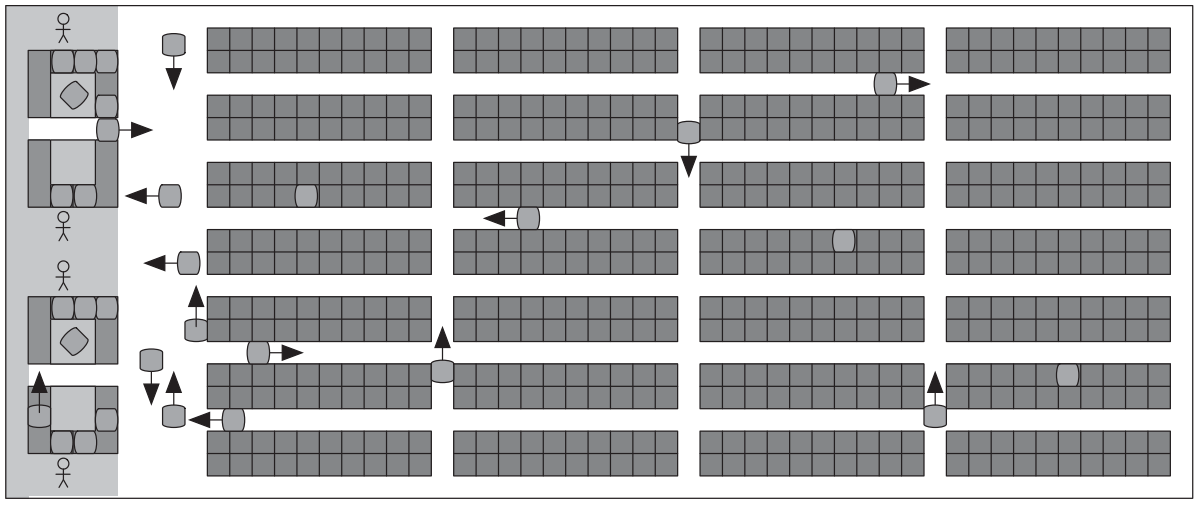
\includegraphics[width=0.9\textwidth]{graphics/kivasystemlayout}
	\caption{A Small Region of a Kiva Layout (\cite{wurman2008coordinating}). Picking stations located on the left and storage pods laid out in rows.}
	\label{kivalayout1}
\end{figure}

\section{Single-agent pathfinding}
Single-agent pathfinding aims to find a path from start node to goal node. In this paper we won't cover the full details of single-agent pathfinding, it has been studying in detail by a number of papers.

The \textit{grid-based path planning competition} (GPPC) is run by \cite{sturtevant2015grid}. The paper provides detailed results of the state of the art at the time in 2015. These are run on a number of game maps which are used for benchmarking \cite{sturtevant2012benchmarks}. While these results are a few years old, we are expecting the results from this year's GPPC.

For our simulation we will aim to assist the MAPF algorithm and will consider looking at two algorithms: \textit{jump point search} and \textit{compressed path databases}.


\section{Multi-agent pathfinding}
Multi-agent pathfinding (MAPF) involves finding a path for every agent to their goal. Warehouse Automation is commonly modeled on an orthogonal undirected grid \cite{TODO}. 


Within MAPF, we are focusing on an optimal solution. The following sections will focus on optimal MAPF algorithms as well as suboptimal variants of these algorithms.


\section{Optimal multi-agent pathfinding algorithms}
Here we look at multi-agent pathfinding algorithms which aim to find the optimal solution based on some objective function. The objective function will be noted per algorithm. Our main aim is to determine the benefits and downsides of each algorithm.


Take a MAPF problem instance where we have $k$ agents on a graph with $n$ nodes. The possible state space is $n^k$ and branching factor is $5^k$. So the complexity of the MAPF problem is exponential in the number of agents and polynomial in the number of nodes on the graph.

a NP-hard problem

Coupled approach: All agents at one! A* ICTS

Decoupled approach: Each agent individually (not optimal, not complete)

\cite{krontiris2013feasibility} looked at the feasibility.

\subsection{Conflict-based Search}
The conflict-based search algorithm (\cite{sharon2015conflict})

Constraint tree.
Conflict tree.

High level: conflict tree

Low level: find optimal paths for each agent

Although CBS is exponential in the number of conflicts, results found that compared against ICTS and A* they suggest it is best in maps with bottlenecks.

\subsection{ICTS}

Exponential in $\Delta$

\subsection{A*}
Exponential in number of agents

\subsection{Push and Rotate}
\cite{wilde2014push}


\section{Bounded suboptimal variants}
A \textit{bounded suboptimal variant} is a variant of an optimal MAPF algorithm. The defining feature of a bounded suboptimal variant is that we can guarantee that the cost of the solution, $B$ lies within the optimal cost $C$ and $w*C$ where $w$ is a user-defined parameter. Hence:

\[C \le B \le w*C\]


Our project is aiming to make a bounded suboptimal variant of our algorithm due to the large-scale of the simulation (Section~\ref{sec:background}). By adjusting $w$ we are able to relax the problem and find a solution faster at the loss of solution quality.

\section{Mixed Integer Programming}
Mixed-integer programming (MIP) is an optimization technique. It looks at an objective function subject to a list of constraints and finds the optimal solution for each variable.

\cite{yu2013planning}


\section{Other reduction-based techniques}
Answer set programming?



\section{Other improvements to Warehouse Automation}
Independence detection

Operator decomposition

\section{Conclusion}


\bibliographystyle{dcu}
\bibliography{bibliography}
	
\end{document}
